\begin{frame}[allowframebreaks]{Low-Rank Adaptation (LoRA)}
\begin{figure}
    \centering
    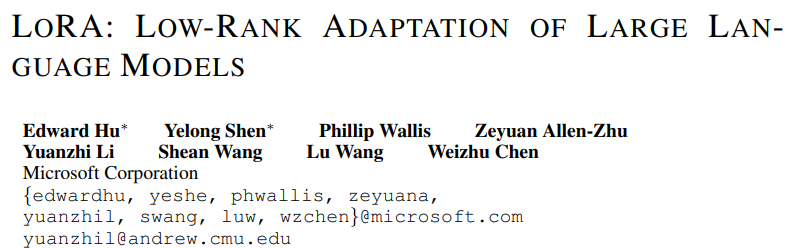
\includegraphics[width=\linewidth,height=\textheight,keepaspectratio]{images/adv-img-gen/lora-1.png}
\end{figure}

\framebreak

\large \textbf{LoRA Overview}\\[0.5ex]
Low-Rank Adaptation (LoRA) is a technique for efficient fine-tuning of large neural networks. Instead of updating all parameters, LoRA injects trainable low-rank matrices into each layer, significantly reducing the number of trainable parameters.

\textbf{Key Idea:} Decompose the weight update $\Delta W$ as a product of two low-rank matrices:
\begin{equation}
    \Delta W = A B
\end{equation}
where $A \in \mathbb{R}^{d \times r}$ and $B \in \mathbb{R}^{r \times k}$, with $r \ll \min(d, k)$.

\framebreak

\begin{figure}
    \centering
    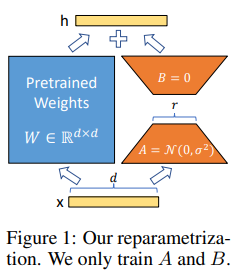
\includegraphics[width=\linewidth,height=0.7\textheight,keepaspectratio]{images/adv-img-gen/lora-2.png} \\
    \small [Hu et al., 2021](https://arxiv.org/abs/2106.09685)
\end{figure}

\framebreak

\large \textbf{LoRA in Linear Layers}\\[0.5ex]
Consider a linear layer with weight $W_0 \in \mathbb{R}^{d \times k}$. In LoRA, the forward pass is modified as:
\begin{equation}
    y = W_0 x + \alpha A B x
\end{equation}
where $\alpha$ is a scaling factor, and only $A$ and $B$ are updated during fine-tuning.

\textbf{Parameter Efficiency:} The number of trainable parameters is reduced from $d \times k$ to $r \times (d + k)$.

\framebreak
\large \textbf{LoRA Training Objective}\\[0.5ex]
The training objective remains the same as standard fine-tuning, e.g., minimizing a loss function $\mathcal{L}$:
\begin{equation}
    \min_{A, B} \mathcal{L}(y, \hat{y})
\end{equation}
where $y$ is the model output and $\hat{y}$ is the ground truth.

\textbf{Regularization:} Optionally, regularization terms can be added to encourage low-rank structure or prevent overfitting.

\framebreak
\large \textbf{LoRA in Attention Mechanisms}\\[0.5ex]
LoRA is commonly applied to the query and value projection matrices in attention layers:
\begin{align}
    Q' &= Q + \Delta Q = Q + A_q B_q \\
    V' &= V + \Delta V = V + A_v B_v
\end{align}
where $A_q, B_q, A_v, B_v$ are low-rank matrices for the query and value projections, respectively.

\framebreak

\begin{figure}
    \centering
    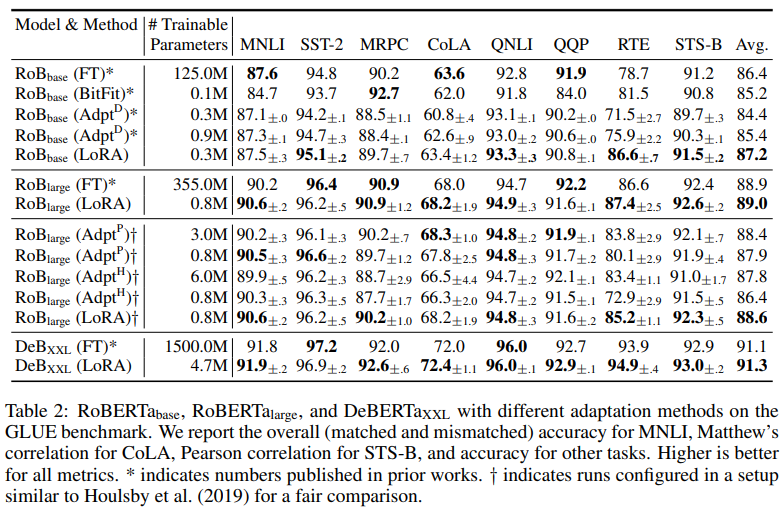
\includegraphics[width=\linewidth,height=0.8\textheight,keepaspectratio]{images/adv-img-gen/lora-3.png} \\
    \small [Hu et al., 2021](https://arxiv.org/abs/2106.09685)
\end{figure}

\framebreak

\begin{figure}
    \centering
    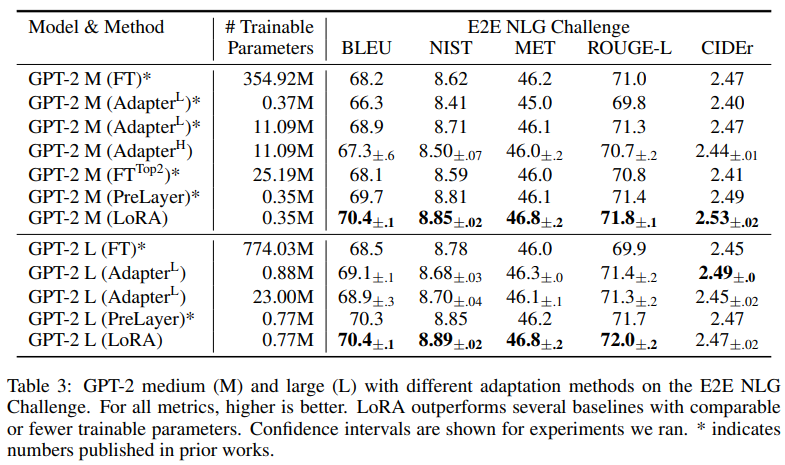
\includegraphics[width=\linewidth,height=\textheight,keepaspectratio]{images/adv-img-gen/lora-4.png} \\
    \small [Hu et al., 2021](https://arxiv.org/abs/2106.09685)
\end{figure}
\framebreak

\begin{figure}
    \centering
    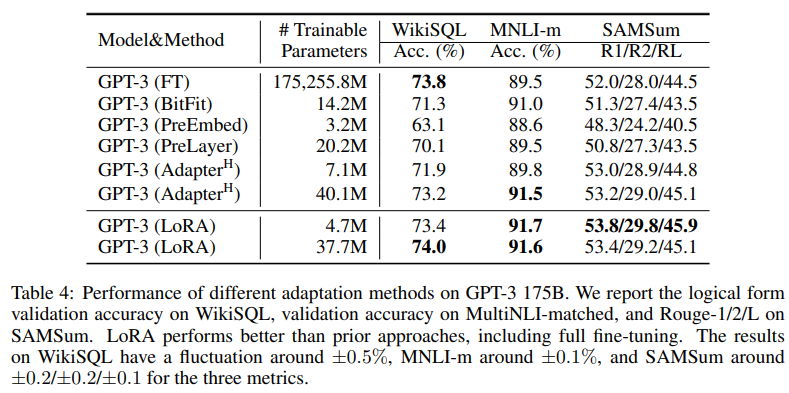
\includegraphics[width=\linewidth,height=\textheight,keepaspectratio]{images/adv-img-gen/lora-5.png} \\
    \small [Hu et al., 2021](https://arxiv.org/abs/2106.09685)
\end{figure}

\framebreak

\begin{figure}
    \centering
    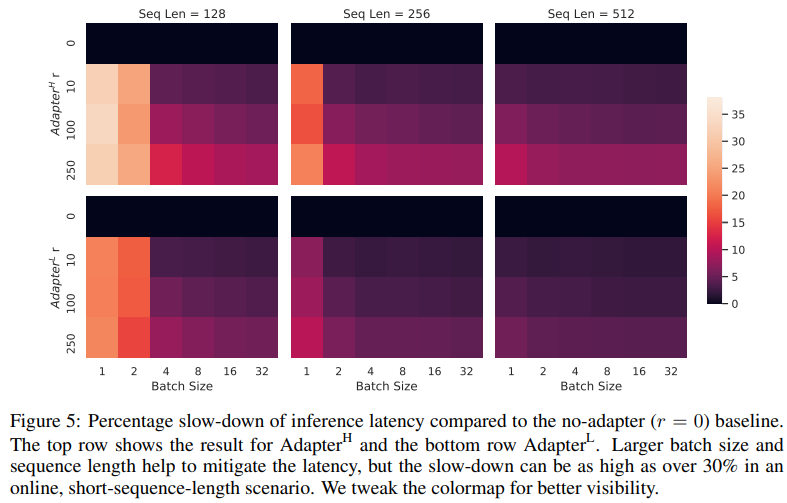
\includegraphics[width=\linewidth,height=\textheight,keepaspectratio]{images/adv-img-gen/lora-6.png} \\
    \small [Hu et al., 2021](https://arxiv.org/abs/2106.09685)
\end{figure}
\end{frame}